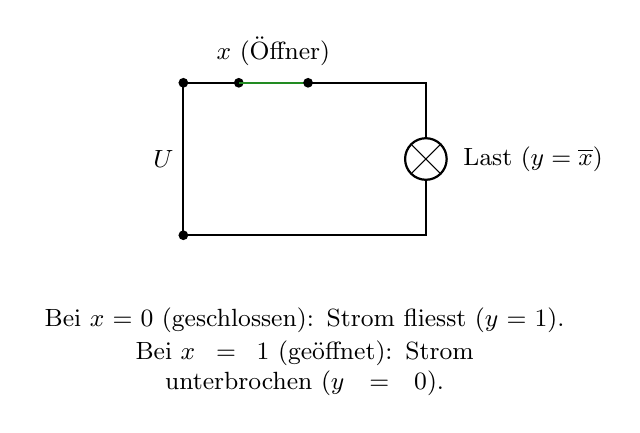
\begin{tikzpicture}[scale=0.88, >=stealth]
    \draw[thick] (0,0) -- (0,2.2) -- (0.8,2.2);
    \node[left, font=\small] at (0,1.1) {$U$};
    \fill (0,0) circle (2pt); \fill (0,2.2) circle (2pt);

    % Öffner-Schalter x
    \fill (0.8, 2.2) circle (2pt);
    \draw[thick, ForestGreen] (0.8, 2.2) -- (1.8, 2.2);
    \node[above, font=\small] at (1.3, 2.3) {$x$ (Öffner)};
    \fill (1.8, 2.2) circle (2pt);
    \draw[thick] (1.8, 2.2) -- (3.5, 2.2) -- (3.5, 1.4);

    % Lampe y
    \draw[thick] (3.5, 1.1) circle (0.3);
    \draw (3.3, 0.9) -- (3.7, 1.3);
    \draw (3.3, 1.3) -- (3.7, 0.9);
    \node[right, font=\small] at (3.9, 1.1) {Last ($y = \overline{x}$)};
    \draw[thick] (3.5, 0.8) -- (3.5, 0) -- (0,0);

    \node[align=center, font=\small, text width=6.8cm, anchor=north] at (1.75, -0.9) {Bei $x=0$ (geschlossen): Strom fliesst ($y=1$).\\[1pt]Bei $x=1$ (geöffnet): Strom unterbrochen ($y=0$).};
\end{tikzpicture}
